\begin{figure}
  \begin{center}
    \begin{tabular}{c}
    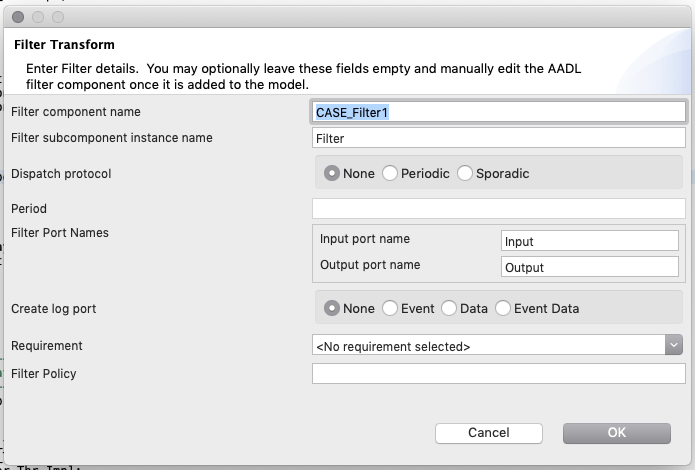
\includegraphics[scale=0.3]{dialogue.png}
    \end{tabular}
  \end{center}
  \caption{BriefCASE dialogue for filter transformation.}
  \label{fig:dialogue}
\end{figure}

\newsavebox{\flt}
\begin{lrbox}{\flt}
  \begin{lstlisting}[style=agree,numbers=left]
    -- start user definitions
    eq policy : bool = 
      WELL_FORMED_AUTOMATION_RESPONSE(Input);
    -- stop user definitions

    guarantee "Filter output is well-formed" :
      if event(Input) and policy then 
        event(Output) and Output = Input
      else 
        not event(Output);
  \end{lstlisting}
\end{lrbox}

\newsavebox{\mntr}
\begin{lrbox}{\mntr}
  \begin{lstlisting}[style=agree,numbers=left]
    const is_latched : bool = true;

    -- start user definitions
    assume "One automation request in flight at a time" : *\label{line:mon-assume}*
      true -> (req => pre(Historically(not req) or Since(not req, rsp)));

    const MAX_LATENCY : int = 1; *\label{line:mon-const}*
        
    eq rsp : bool = event(Response);
    eq req : bool = event(Request);

    eq isPending : bool = Since(not rsp, req and not rsp);*\label{line:mon-pending}*
    eq latency : int = 0 -> (if req then 0 else pre(latency) + 1);*\label{line:mon-latency}*
    
    eq policy : bool = (rsp => req) -> *\label{line:mon-policy}*
                         (    (isPending => latency < MAX_LATENCY)   
                          and (rsp => (req or pre(isPending))));
    -- stop user definitions
    
    eq alert : bool = (not policy) -> *\label{line:mon-alert}*
                        ((is_latched and pre(alert)) or not policy);
                          
    guarantee "Alert port tracks alert variable" :
      event(Alert) = alert;
    guarantee "Output if not alerted" :
      if (not(alert) and rsp) then
          event(Output) and (Output = Response)
      else
          not (event(Output));    
  \end{lstlisting}
\end{lrbox}

\begin{figure}
  \begin{center}
    \begin{tabular}{c}
      \scalebox{0.62}{\usebox{\flt}} \\
    \end{tabular}
  \end{center}
  \caption{Contract specification for high-assurance filter.}
  \label{fig:filter}
\end{figure}

\begin{figure}
  \begin{center}
    \begin{tabular}{c}
    \scalebox{0.62}{\usebox{\mntr}} \\
    \end{tabular}
  \end{center}
  \caption{Contract specification for high-assurance monitor.}
  \label{fig:monitor}
\end{figure}

As noted previously, the system with the untrusted AI does not pass AGREE verification.
Transformations in BriefCASE are used to cyber-harden the system against malicious AI behavior by inserting a high-assurance filter and monitor between the AI and the WM as shown in \figref{fig:hardened}.
High-assurance means the behaviors of the components are verified.
Here the filter protects the WM from malformed data and the monitor protects it from spontaneous or delayed responses.
These high-assurance components are added one at a time by selecting the connection in the model where the component is to appear and then choosing the appropriate transformation.

The system designer provides configuration parameters for the transformation in a dialogue box.
The dialogue box for adding a filter is shown in \figref{fig:dialogue}.
All high-assurance components rely on a \emph{policy} to define behavior as seen in the last field of the dialogue box.
A filter policy defines well-formed data while a monitor policy defines an invariant over inputs and outputs.
These policies can be stated directly in the wizard, or they can be left blank and added later to the AGREE contract generated by the transformation.

BriefCASE creates all the needed AADL for the new high-assurance component and its connections in the system implementation as part of the transformation.
It also creates a default AGREE specification that defines everything about the component behavior but the policy itself unless it is provided in the dialogue.
The resulting AGREE specification from the transformation for the filter is shown in \figref{fig:filter}.
The single guarantee completely defines the filter output under any input according to the truth value of the policy.
While such a strong guarantee is not required for AGREE analysis, it is required for automated synthesis.

The AGREE specification for the monitor is shown in \figref{fig:monitor} and is considerably more complex than the filter.
BriefCASE generates everything but the statements in \linesref{line:mon-assume}{line:mon-policy}.
As with the filter, the guarantees completely define the output, as required for synthesis, in terms of the policy and the alert.
The \texttt{alert} variable defined on \lineref{line:mon-alert} depends not just on the policy but also on the indicated behavior from the BriefCASE dialogue box. 
Marking \texttt{is\_latched} as true makes the alert persistent, meaning that once the alert is raised, it is always raised; otherwise, it is the complement of the policy value in the current step.

The monitor policy is defined by marking when a request is not satisfied, \texttt{isPending} on \lineref{line:mon-pending}, and counting the number of steps between requests, \texttt{latency} on \lineref{line:mon-latency}.
The \texttt{isPending} variable is true whenever there is a request that does not coincide with a response--\emph{not response since request and not response}.
The \texttt{latency} variable starts at zero, resets on every request, and otherwise increments by one.

The latency bound for the monitor is defined by the constant \texttt{MAX\_LATENCY} on \lineref{line:mon-const}.
Here the constant is set to one to be consistent with the system specification from the previous section.
At time 0 the policy is trivial: a response requires an accompanying request.
After time 0, if a request is pending in the current time step, then the latency must still be under the bound, and if there is a response, then it closes a request now or a pending request from earlier in time.

The policy definition only works if there is never more than one outstanding request at a time; otherwise, the latency counter resets incorrectly.
That requirement is encoded in the assumption on \lineref{line:mon-assume} and is the same assumption used for the system input.
The policy can be written without needing the assumption, but it is much simpler to write with the assumption.

As shown in \figref{fig:hardened-certificate}, the cyber-hardened system passes AGREE verification.
That means that the high-assurance components protect the WM from the untrusted AI generating malformed data, spontaneous responses, or delayed responses.
Synthesis must generate precise implementations of the high-assurance component specifications for the AGREE verification result to apply to the deployed system.
Precise in this context means that the implementations match the input to output relations defined in the specifications.
